\section {Разработка программного комплекса}
В данном разделе описывается процесс проектирования и разработки комплекса алгоритмов и программ для численного исследования процессов, протекающих в системах массового обслуживания, а также расчетов характеристик их функционирования. Ключевой составляющей данного комплекса является имитационная модель. Также программный комплекс содержит утилиты для вычисления дискретного преобразования Фурье, расчета расстояния Колмогорова, а также параметризованное решение системы уравнений Колмогорова для вычисления асимптотического приближения характеристической функции числа обслуженных заявок в системе массового обслуживания с повторными вызовами и обратной связью \cite{blaginin2021approximation}.

Проектирование программы начинается с разработки архитектуры по предварительно составленным требованиям. В данном случае, делается упор на универсальность модели и возможность встраивания ее в непосредственный процесс анализа. Также особое внимание уделяется процедуре проведения численных экспериментов. Численные результаты являются наиболее репрезентативными в случае, если было проведено достаточное количество экспериментов при наборах параметров, которые описывают функционирование модели в различных ситуациях. Такой подход позволяет удостовериться в верности теоретической стороны исследования посредством анализа объемной выборки данных о работе модели.

Архитектура программы была разработана с учетом следующих требований к ее работе и процессу взаимодействия с пользователем. Требования были составлены исходя из имеющегося опыта анализа систем массового обслуживания при помощи имитационного моделирования и опираясь на реализации имеющихся инструментов \cite{yakimov2017comparison}:
\begin{enumerate}
	\item производительность. Инструмент должен обладать достаточным быстродействием, чтобы в течение адекватного времени (от нескольких минут до пары часов) проводить имитационное моделирование даже на домашнем компьютере. Данное требование также обосновано необходимостью получать объемные выборки для получения достоверных результатов моделирования;
	\item универсальность. Возможность моделирования широкого спектра моделей теории массового обслуживания;
	\item инструмент должен иметь возможность проведения масштабных экспериментов. Другими словами, программа должна быть оптимизирована для запуска большого количества моделей параллельно;
	\item параметризация. Возможность настройки как работы элементов модели в отдельности так и модели в целом, что включает подбор типа распределения генерируемых задержек, самих параметров распределения и условного времени моделирования;
	\item возможность производить сбор данных о работе модели в требуемом контексте. Иначе говоря, инструмент должен позволять собрать конкретные статистические данные имитационного моделирования в зависимости от поставленной задачи;
	\item интеграция в процесс анализа. Другими словами, имитационное моделирование должно быть одним из инструментов среды, в которой проводится анализ. Из данного требования вытекает и выбор целевой программной среды для разработки, чтобы обеспечить легкость установки и начала использования программы в независимости от платформы;
	\item легкая расширяемость. Исходный код программы должен предоставлять возможность добавления новой логики.
\end{enumerate}

\subsection{Предметная область}
Исходя из выше представленных требований, инструмент должен иметь возможность производить моделирование различных систем массового обслуживания. Наиболее гибким вариантом реализации данного требования будет включить построение модели в процесс работы с инструментом. Так, у пользователя появляется возможность конфигурировать требуемую под задачу систему массового обслуживания.

Для достижения предложенного подхода предлагается использовать конструирование блоками \cite{valentin2002simulation} --- инструмент будет включать в себя набор атомарных элементов систем массового обслуживания (обслуживающий прибор, входящий поток и т.д.), которые будут работать по принципу черного ящика, однако связь между элементами и промежуточные этапы будут доступны для конфигурирования. Такой подход позволяет создать абсолютно любую вариацию системы массового обслуживания и используется не только в имитационном моделировании. Зачастую подобное архитектурное решение можно наблюдать в программных комплексах, предназначенных для программирования сложных взаимодействий между объектами. В 3D--графике зачастую используется схожий процесс работы, основанный на графах, где вершины представляют собой алгоритмы и объекты, а ребрами являются взаимодействия между ними. Например, в ПО для создания эффектов и симуляции взаимодействия физических тел Houdini используется именно такой подход \cite{claes2009controlling}.

Принцип работы имитационной модели базируется на обработке событий, происходящих в системе во время ее функционирования. Под событиями понимаются перемещения заявок по элементам системы. Обработка включает в себя регистрацию времени наступления события. Заявками же являются объекты, которые обрабатываются в ходе работы системе. Цикл обработки заявки, как правило, начинается с поступления ее в систему из входящего потока, далее поступление на прибор, обслуживание и последующее покидание системы. Именно из особенностей прохождения заявок через систему складываются характеристики ее функционирования.

Для разработки инструмента выбран объектно--ориентированный подход. Его преимуществом является возможность построения абстракций над логикой работы конкретных элементов системы, что позволяет удовлетворить требованию легкой расширяемости и позволить конструирование модели блоками в процессе анализа. 

Объектно--ориентированный подход \cite{fowler1997analysis} к реализации предметной области подразумевает выделение из нее отдельных сущностей, которые могут быть представлены одним самостоятельным объектом, выполняющим конкретную задачу.

Процесс моделирования заключается в перемещении заявок от одного элемента к другому. В очередной условный момент времени $T_{cur}$ местонахождение каждой заявки и ее характеристики могут меняться. По этой причине для каждой заявки вводится условный момент времени моделирования, когда она изменит своё состояние --- $T_{shift}$. В момент времени, когда $T_{shift} = T_{curr}$, заявка перемещается в очередной элемент модели, и  $T_{shift}$ обновляется им в зависимости от заданных параметров. Иначе процесс моделирования можно представить как последовательное изменение состояния системы, складывающегося из текущих состояний ее элементов. В свою очередь события, происходящие в системе могут быть поделены на несколько основных категорий:
\begin{enumerate}
	\item прибытие заявки в систему;
	\item начало обслуживания заявки на приборе;
	\item окончание обслуживания заявки на приборе;
	\item перемещение заявки в источник повторных вызовов (орбиту, при ее наличии в системе);
	\item попытка повторного обращения из источника повторных вызовов.
\end{enumerate}

В первую очередь, как ранее было указано, выделим элемент модели --- объект, который содержит некую вычислительную логику и обрабатывает заявки в соответствии с этой логикой. Примером элемента модели является обслуживающий прибор.

Для того, чтобы соединить элементы в единую модель, потребуется определенном образом указать, как заявки будут перемещаться между элементами. Для этой цели выделим сущность --- маршрутизатор. Однако в зависимости от реализации элемента, он может иметь разное количество связей, с помощью которых будут перемещаться заявки. Таким образом, требуется ввести сущность, которая регулирует количество и качество возможных соединений элемента --- слот.

Заявка также представлена сущностью, которая хранит в себе время смены ее состояния на новое, текущее состояние и другие опциональные атрибуты.

Поскольку элемент модели работает по принципу черного ящика, то не следует отягощать его логику сбором данным о моделировании. Для этой цели можно использовать маршрутизатор, отслеживая характеристики перемещения заявок в нужных участках модели. Исходя из этого, логику сбора статистики можно вынести в отдельную сущность, что позволит добавить в данный процесс разнообразную логику.

Итак, в предметной области программы были выделены следующие сущности:
\begin{itemize}
	\item элемент системы --- объект, являющийся частью модели и выполняющий обработку заявок на протяжении ее работы;
	\item заявка --- объект, перемещающийся по системе и подлежащий обработке;
	\item маршрутизатор --- объект, образующий односторонний туннель для перемещения заявок от элемента системы к другому;
	\item слот --- объект, служащий для соединения двух элементов при помощи маршрутизатора;
	\item сборщик статистики --- объект, собирающий данные о перемещении заявок по маршрутизатору;
	\item генератор задержки --- объект для генерации случайных величин с требуемым распределением.
\end{itemize}

\subsection{Объектная модель предметной области}
На основе выделенных сущностей и описанного принципа работы программы была построена ее объектная модель, впоследствии использованная для реализации. Для графического представления предметной области используется язык моделирования UML \cite{pilone2005uml}, в частности диаграмма классов \cite{herchi2012user}, позволяющая графически изобразить выделенные в предметной области сущности в качестве классов и взаимосвязь между ними.

Для обеспечения универсальности и возможности добавления новых разновидностей элементов модели был введен общий для них интерфейс Producer. Такое решение, в качестве побочного эффекта, также может позволять использовать различные элементы системы в несвойственных для них позициях в модели.
\begin{figure}[H]
	\centering
	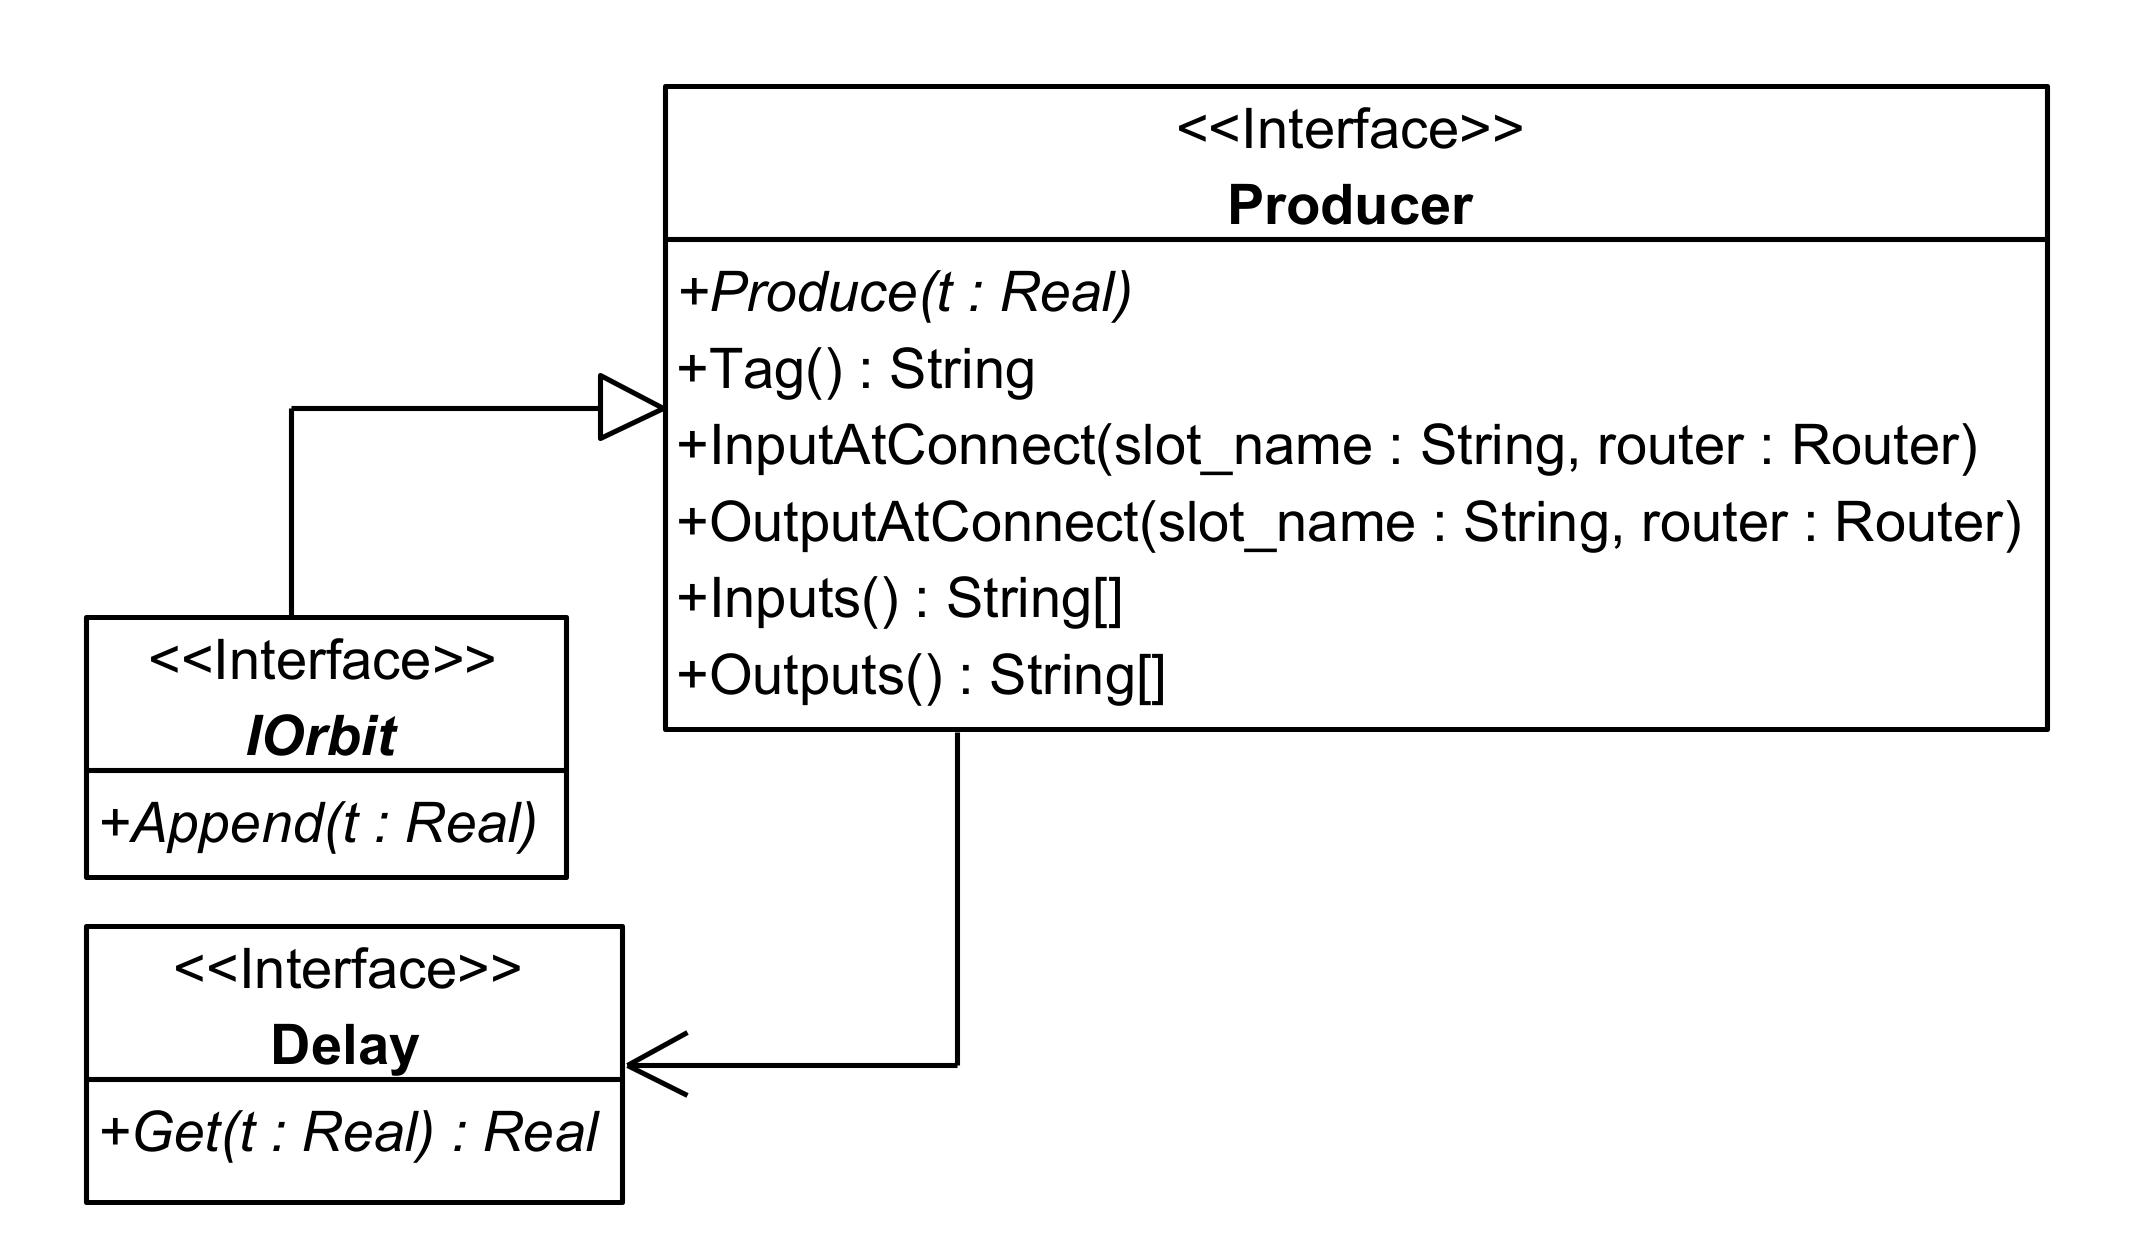
\includegraphics[scale=0.3]{d_producer.png}
	\caption{Интерфейс Producer}
	\label{d_producer}
\end{figure}

В абстрактном методе Produce должна находится логика работы элемента системы, и именно этот метод будет вызываться в каждой итерации работы модели, возвращая вектор моментов времени наступления событий в элементе. Также в интерфейсе определены вспомогательные методы Tag, InputAtConnect, OutputAtConnect, Inputs и Outputs, служащие для соединения элементов между собой. Метод Tag возвращает константную строку, определенную для каждой реализации интерфейса Producer. Слоты элемента разделена на два класса --- входящие, которые позволяют принимать элементу заявки, и выходящие, позволяющие ему их отправлять. Методы InputAtConnect и OutputAtConnect позволяют присоединять к маршрутизатору входящие и выходящие слоты соответственно, указывая название слота для соединения. 

Другим важным элементом предметной области является объект, генерирующий время задержки заявок в процессе их перемещения и позволяющий проводить эксперименты, когда элементы системы могут задавать задержку для заявки разного рода. Для этой цели служит интерфейс Delay. Он имеет единственный метод Get, возвращающий сгенерированную случайную величину.
\begin{figure}[H]
	\centering
	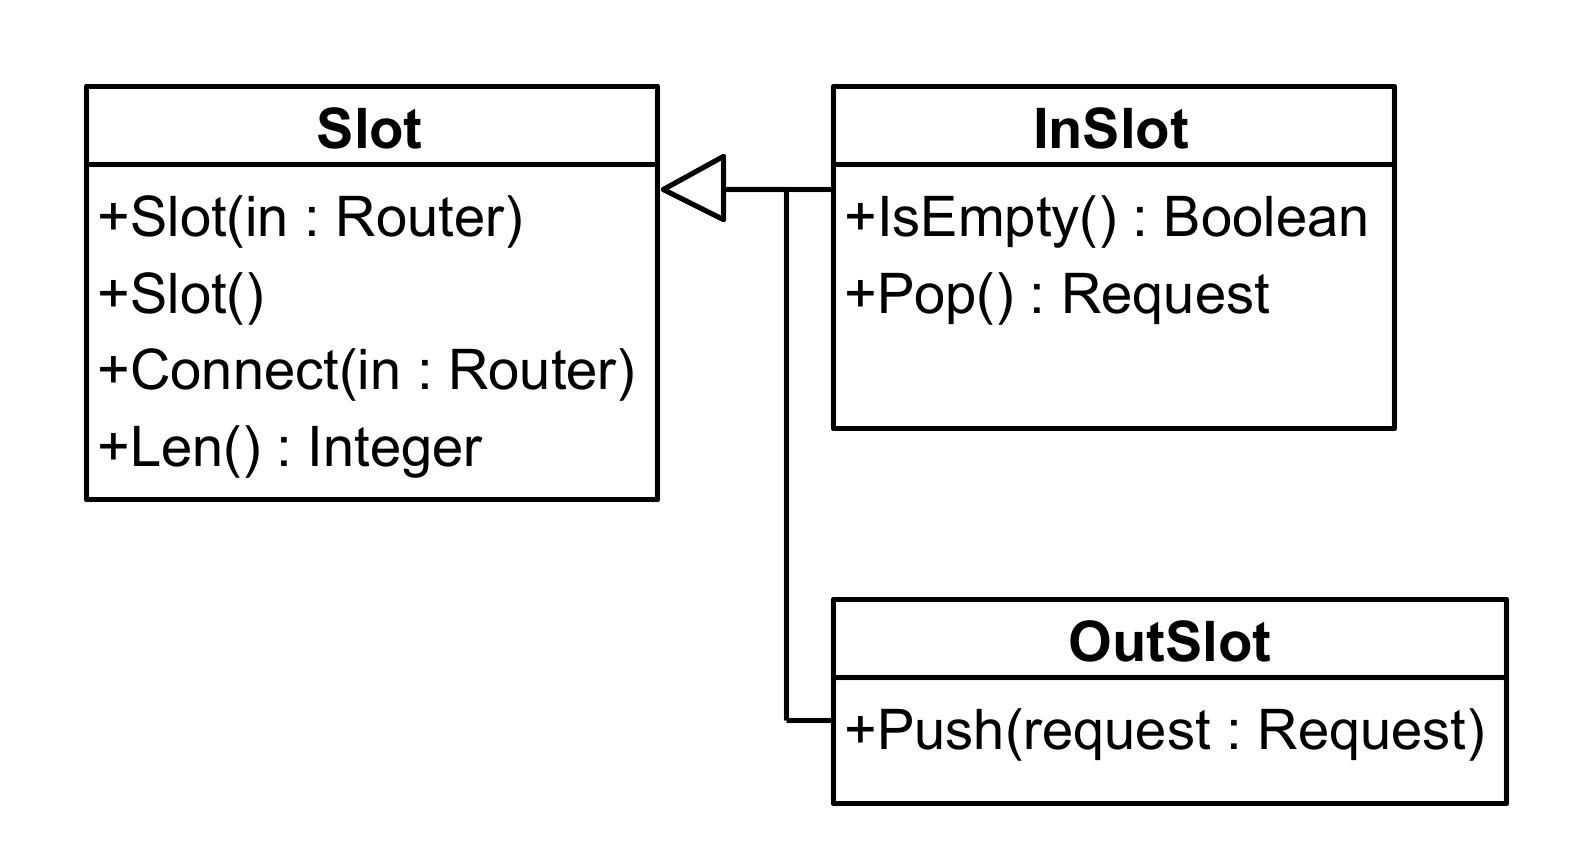
\includegraphics[scale=0.3]{d_slot.png}
	\caption{Класс Slot и его наследники}
	\label{d_slot}
\end{figure}

Слоты используются в элементах системы для задания ограничения на возможные связи между другими элементами. К примеру, входящий поток может иметь только один выход для заявок, которые им генерируются, и не имеет входов, поскольку порождает заявки самостоятельно. В свою очередь, орбита должна иметь один вход для поступающих на нее заявок и один выход для отправления их обратно. Для разграничения логики работы слота на принимающий и отправляющий введено два наследника --- InSlot, способный только принимать заявки при помощи метода Pop и OutSlot, предназначенный лишь для их отправления при помощи метода Push. Среда для переправки заявок между слотами обеспечивается за счет класса Router.

\begin{figure}[H]
	\centering
	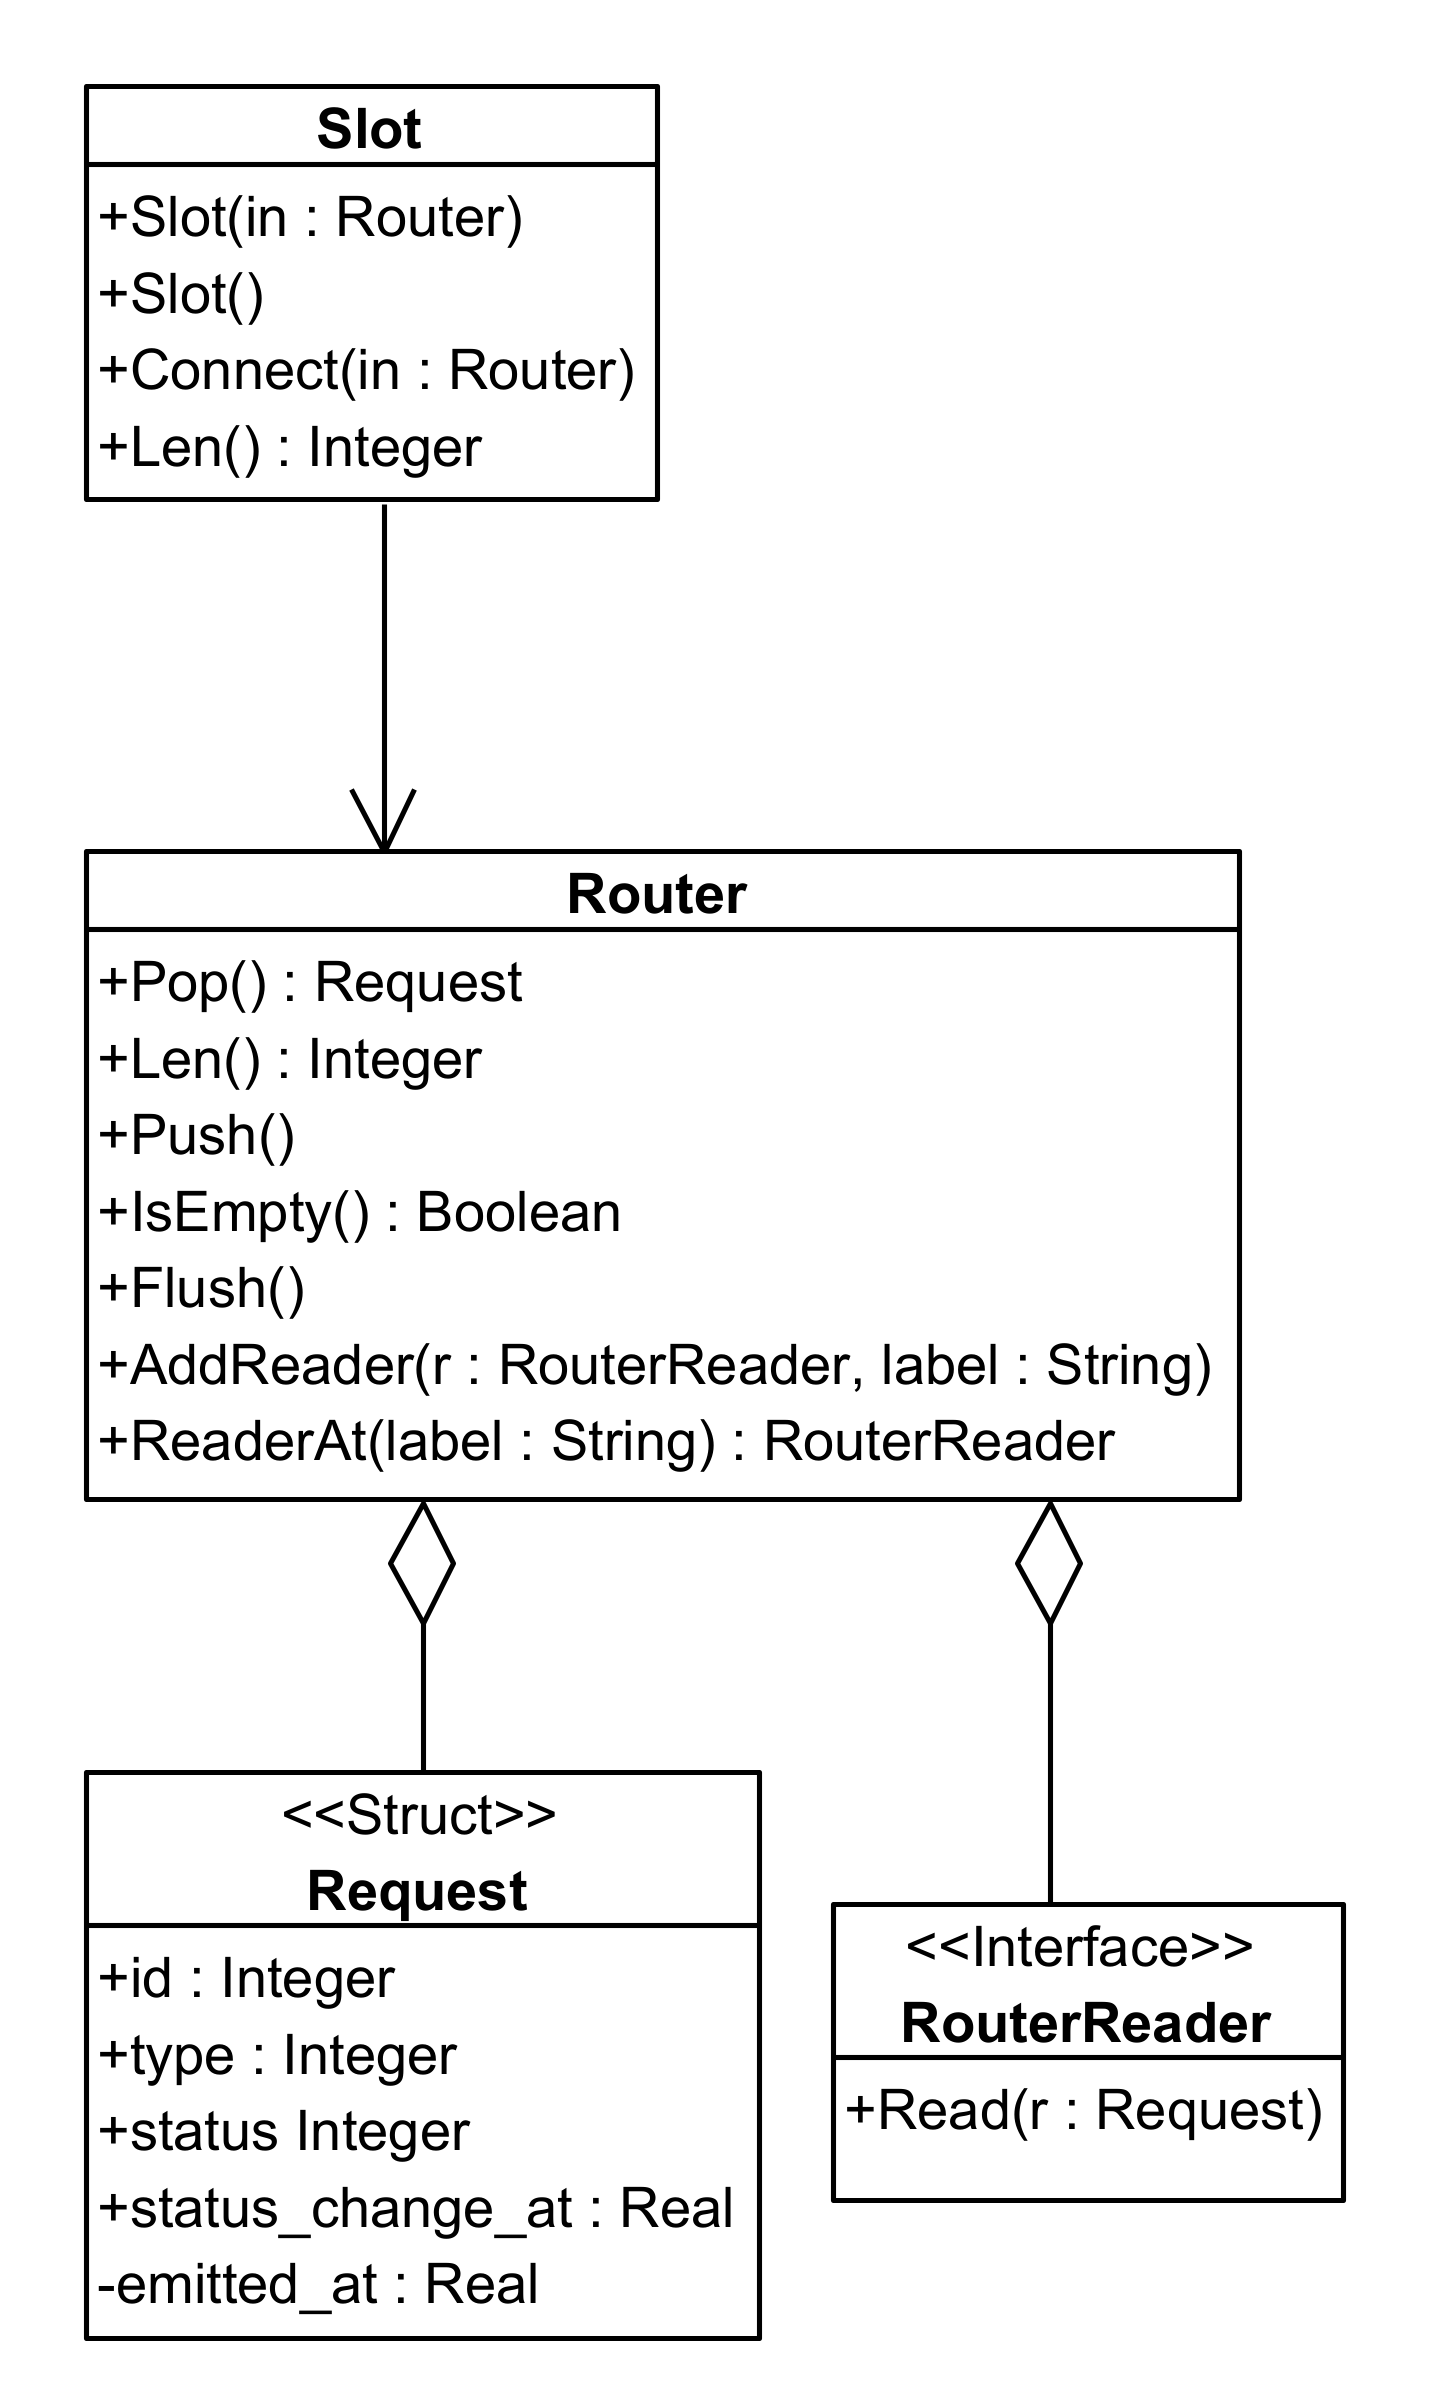
\includegraphics[scale=0.3]{d_router.png}
	\caption{Класс Router}
	\label{d_router}
\end{figure}
Маршрутизатор представляет собой очередь, работающую по принципу FIFO. Таким образом, он позволяет элементам системы взаимодействовать с заявками между итерациями, когда очередная заявка еще ожидает обработки, но текущая итерация подошла к концу. Управление очередью заявок осуществляется при помощи методов Push (поместить заявку в очередь), Pop (достать заявок из очереди), Len (получить текущую длину очереди), IsEmpty (пуста ли очередь). Методы AddReader и ReaderAt предназначены для управления набором сборщиков статистики. AddReader позволяет добавить новый сборщик статистики под указанным ярлыком, который позволит обращаться к нему в последствии при помощи метода ReaderAt для доступа к собранным данным.

Заявка представлена структурой Request, содержащей момент изменения ее состояния status\_change\_at ($T_{shift}$), тип, служащий для разделения способа происхождения заявки, статус, отражающий этап ее обработки (обслужена, в процессе обслуживания, в пути, покинула систему) и время, когда заявка была создана.

Ниже представлена полная объектная модель предметной области, объединяющая ранее представленные классы и интерфейсы.
\begin{figure}[H]
	\centering
	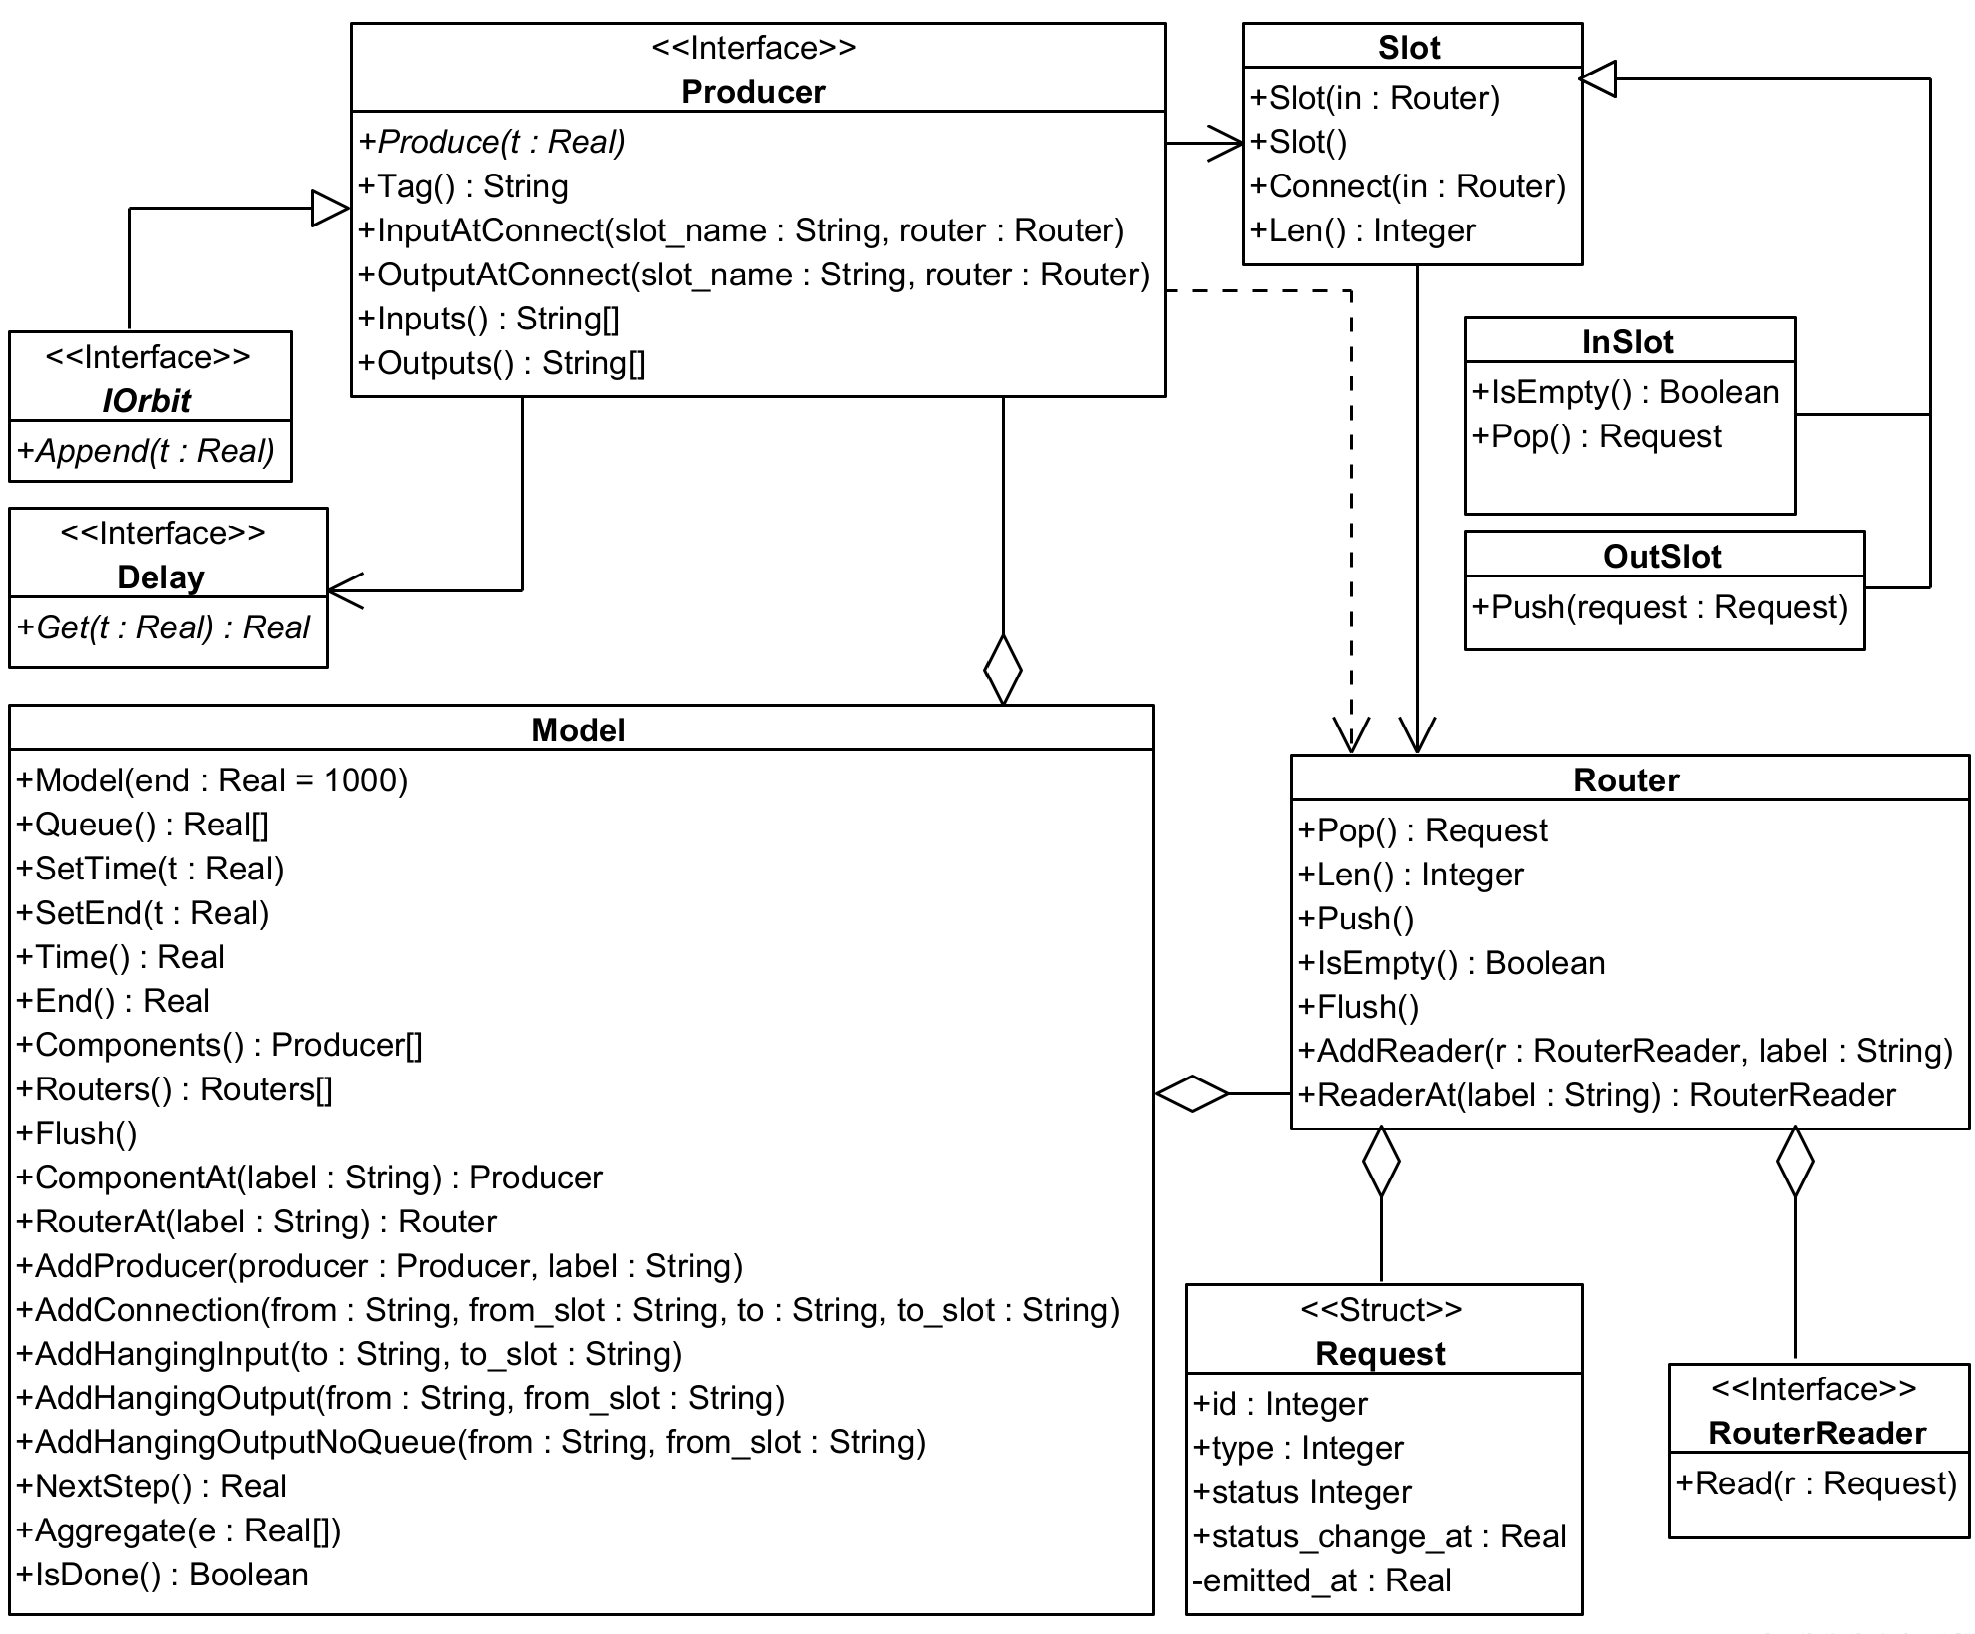
\includegraphics[scale=0.3]{d_d.png}
	\caption{Объектная модель предметной области}
	\label{d_d}
\end{figure}

Как видно на рисунке \ref{d_d}, предметная область содержит специальный агрегирующий класс Model, предназначенный для управления процессом моделирования в рамках одной системы. Он позволяет построить модель при помощи методов AddProducer (добавление нового элемента в модель) и AddConnection (добавление маршрутизатора между существующими элементами).

AddConnection имеет три частных случая: AddHangingInput --- добавляет маршрутизатор на входящий слот одного элемента, AddHangingOutput --- добавляет маршрутизатор на выходящий слот элемента, AddHangingOutputNoQueue --- аналогичен AddHangingOutput, но заявки не сохраняются в маршрутизаторе. Три перечисленных метода позволяют вручную отправлять заявки в модель, а также устанавливать поток заявок между отдельными моделями.

Метод Queue возвращает текущий вектор моментов наступления событий в системе. SetTime, Time, SetEnd, End устанавливают либо возвращают текущее условное время и условное время окончания моделирования соответственно. Методы Components и Routers возвращают список имеющихся в модели элементов и маршрутизаторов соответственно. Методы ComponentAt и RouterAt предоставляют доступ к конкретному элементу или маршрутизатору. Метод Aggregate добавляет в вектор предстоящих событий новые, а метод NextStep сдвигает время моделирования на момент наступления ближайшего события и возвращает его. Метод IsDone позволяет узнать, закончилось ли моделирование (текущее время моделирования стало равно времени окончания моделирования).

Иначе содержимое модели можно представить графически следующим образом (рисунок \ref{model_container}):
\begin{figure}[H]
	\centering
	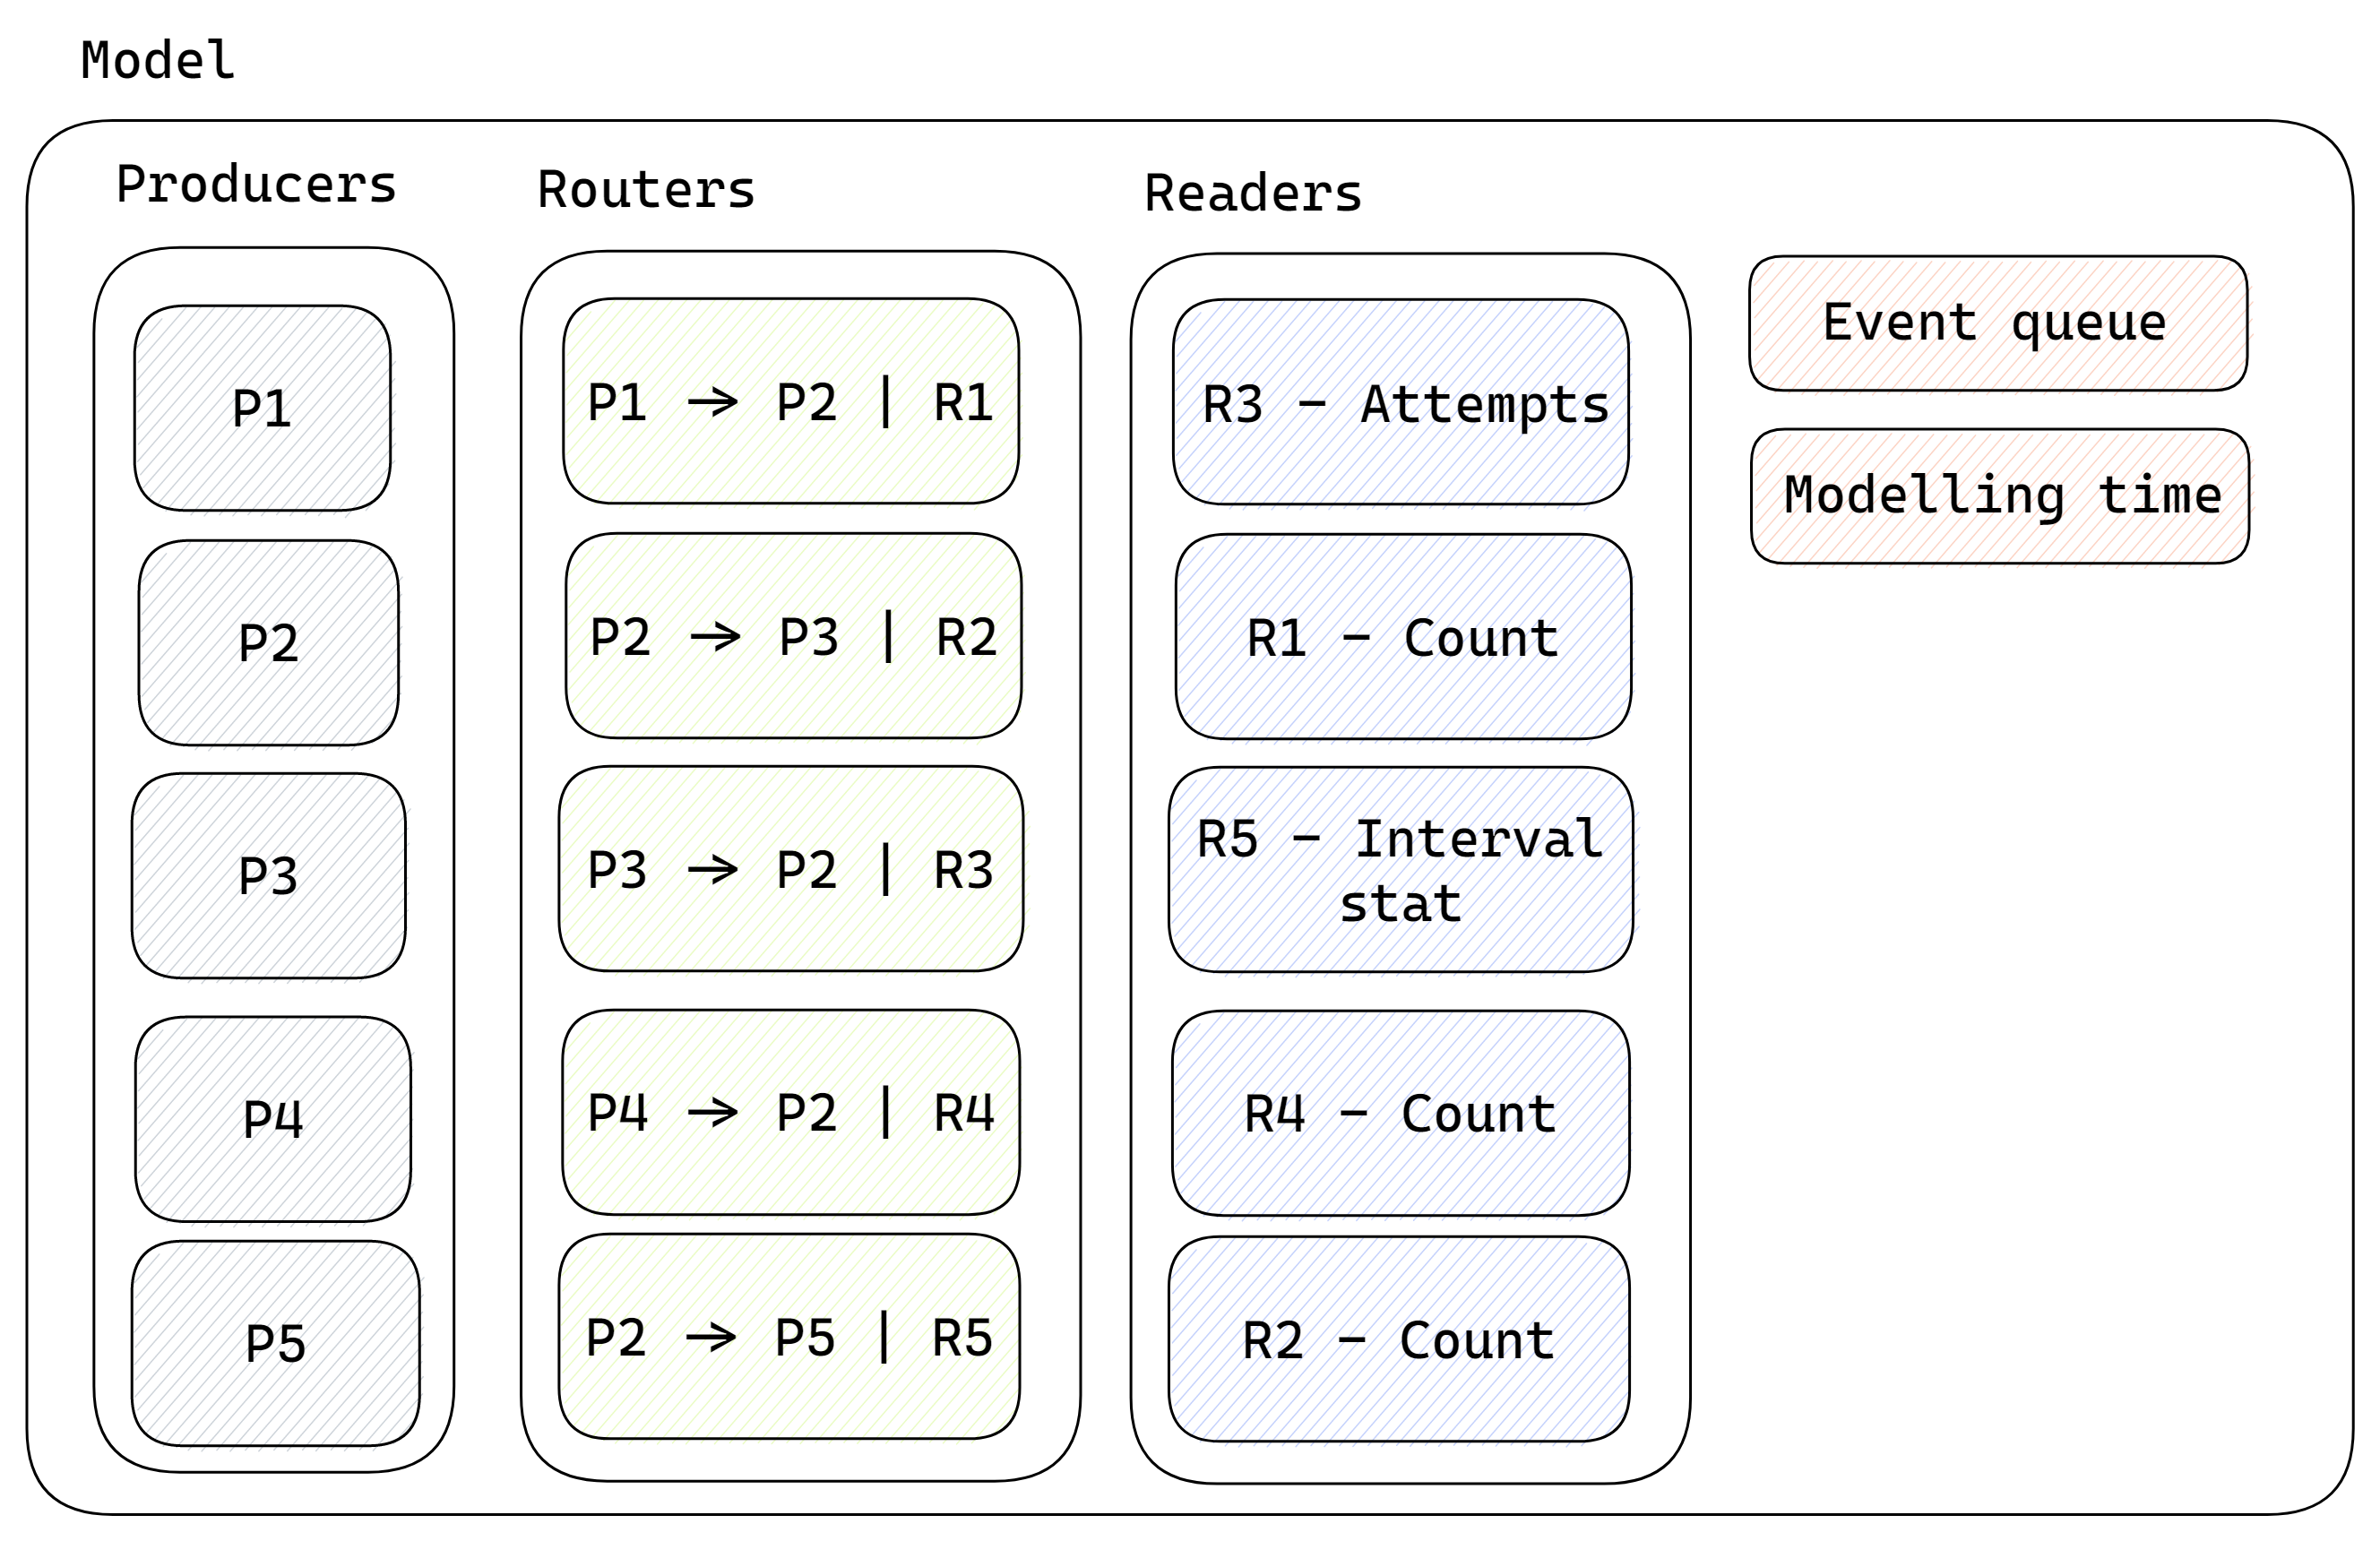
\includegraphics[scale=0.18]{model_container.png}
	\caption{Объектная модель предметной области}
	\label{model_container}
\end{figure}

\subsection{Реализации интерфейсов}
В данном разделе представлены имеющиеся реализации интерфейсов и родительских классов, описанных ранее в предметной области, но не представленных на рисунке \ref{d_d}. Интерфейсы были выделены таким образом, чтобы предоставить возможность к легкому расширению имеющейся реализации. Поскольку логика работы каждого элемента модели, генератора задержек и сборщика статистики не зависит от реализации других элементов того же семейства классов, это позволяет без труда создавать новые элементы со сложной логикой без надобности изменения имеющихся реализаций. Наглядным примером данной особенности является интерфейс Producer, предназначенный для работы в качестве элемента модели. Для него существует три ряда реализаций, разделенных по предназначению. 

Первым классом являются обслуживающие приборы. Среди них:
\begin{enumerate}
	\item SimpleNode --- реализация простейшего обслуживающего прибора, который обслуживает входящие заявки и передает их далее. В случае, если заявка не может получить доступ к прибору, она теряется;
	\item RQNode --- реализация обслуживающего прибора с орбитой. Функционирует аналогично простейшему прибору, однако заявки, не сумевшие попасть на прибор перемещаются на орбиту, откуда снова пытаются захватить его;
	\item RQTNode --- аналогичен прибору с орбитой, но обслуживает два типа заявок: входящие и приходящие из источника повторных вызовов.
\end{enumerate}


Далее описаны источники заявок --- объекты, имеющие только выход для порожденных заявок:
\begin{enumerate}
	\item SimpleInput --- реализация пуассоновского потока;
	\item MMPPInput --- служит для имитации работы Марковского модулированного пуассоновского процесса (MMPP). Для этого имеет поля, содержащие матрицу инфинитезимальных характеристик, вектор интенсивностей для каждого состояния, текущие состояние управляющей цепи, момент времени смены состояния управляющей цепи, а также метод для смены ее состояния shift. Позволяет моделировать ситуации, когда в системе периодически может случаться резкий всплеск заявок, например в реальной жизни пример работы MMPP будет являться резкий наплыв пользователей на интернет ресурс в час пик.
\end{enumerate}

Для орбиты имеется лишь одна реализация через наследованный от Producer интерфейс IOrbit, позволяющий при помощи отдельного метода вводить заявки на орбиту и рассчитывать их время нахождения там.

Отметим, что каждая из реализаций имеет в качестве параметра генераторы случайных задержек, что позволяет существенно менять характеристики функционирования элемента. Для этого интерфейса (Delay) имеются следующие реализации:
\begin{enumerate}
	\item ExponentialDelay --- генератор экспоненциально распределенного времени задержки;
	\item UniformDelay --- генератор равномерно распределенного времени задержки;
	\item GammaDelay --- генератор задержки, имеющей гамма распределение;
 	\item WeibullDelay --- генератор задержки, имеющей распределение Вейбулла \cite{hallinan1993review};
 	\item LognormalDelay --- генератор задержки, имеющей логнормальное распределение.
\end{enumerate}

Для маршрутизатора, помимо основной реализации, имеются два особых случая:
\begin{enumerate}
	\item NoneRouter --- очередь всегда пуста, а заявки, попадающие в нее, уничтожаются. Данный класс предназначен для тех случаев, когда заявки надо направить в тупик после обслуживания и их учет не требуется;
	\item OutputRouter --- отличается от NoneRouter тем, что учет проходящих по очереди заявок ведется, однако они по-прежнему не хранятся.
\end{enumerate}

Сборщики статистики:
\begin{enumerate}
	\item IntervalRouterReader --- сборщик статистики, класс для сбора информации о выходящих процессах системы. Имеет методы и поля для расчета характеристик ее работы, таких как среднее число обслуженных вызванных пришедших заявок, расчет двумерного, суммарного распределения, а также распределений выходящего процесса, обслуживающего входящие заявки и процесса, обслуживающие вызванные заявки. Также имеются методы, позволяющие рассчитать вариацию длин интервалов между моментами завершения обслуживания заявок для каждого из выходящих процессов;
	\item AttemptCounter --- сборщик, учитывающий количество раз, которое каждая заявка прошла через маршрутизатор, а также суммарное время, потраченное на перемещение до цели;
	\item TimeCounter --- сборщик, учитывающий моменты времени, когда заявки проходили через маршрутизатор.
\end{enumerate}

\subsection{Особенности реализации}
В данном разделе описаны подробности реализации имитационной модели.

 Исходный код, реализующий предметную область, выполнен на языке программирования C++ стандарта 2020 года (C++2a). Выбор в сторону C++ был сделан исходя из требований к инструменту, которые включают производительность и возможность интеграции непосредственно в процесс исследования, о чем подробнее изложено ниже. C++ отлично подходит для написания производительного программного обеспечения, а также обеспечивает гибкость в плане архитектурных решений и управления памятью. Помимо этого, С++ является объектно--ориентированным языком программирования, что важно для реализации предметной области. Однако с некоторыми различиями, такими, как отсутствие интерфейсов в явном виде. Вместо них C++ поддерживает абстрактные классы с чистыми виртуальными функциями \cite{schmid2012c++}.
 Также важными аспектами являются:
 \begin{enumerate}
 	\item ручное управление памятью. С одной стороны, необходимость постоянно следить за выделяемой памятью и разрушением экземпляров объектов является недостатком, так как осложняет процесс разработки и способствует возникновению ошибок в управлении памятью, с другой --- дает возможность организовать подходящий под задачу процесс выделения памяти;
 	\item компиляция. Компилируемые языки всегда превосходят в производительности интерпретируемые, поскольку проверка типов, предупреждение возникших исключений и других ошибок происходят на этапе компиляции, а не в процессе работы программы;
 	\item статическая типизация. Заранее известные типы объектов ускоряют как компиляцию, так и работу программы ввиду отсутствия проверки типов;
 	\item объявление без инициализации. C++ позволяет объявить переменную, не инициализируя ее некоторым значением, что экономит время работы.
 \end{enumerate}

 Для сборки программы использовался компилятор GCC \cite{gcc}, поскольку он поддерживается всеми платформами, а также имеет широкий спектр параметров для оптимизации кода на этапе компиляции \cite{branco2015impact}. 
 
 Также стоить отметить подход к генерации случайных величин во время моделирования. Поскольку получаемые величины по своей природе являются псевдослучайными, то генерируются они с использованием в качестве параметров такта центрального процессора или системного времени. При использовании такого генератора во время имитационного моделирования получаемые данные будут недостоверны, поскольку генерация будет производится крайне часто --- для каждого элемента модели в каждой итерации, что вызовет появление повторяющихся значений в генерируемой последовательности чисел. Для решения данной проблемы используется вихрь Мерсенна \cite{matsumoto1998mersenne} --- алгоритм генерации псевдослучайных чисел, основывающийся на свойствах простых чисел Мерсенна. Алгоритм гораздо менее предсказуем, имеет большой период повторения и полное отсутствие статистической закономерности. 
 
 В стандартной библиотеке C++ имеется реализация вихря Мерсенна под названием MT19937 \cite{mersenn}, где число в названии связано с величиной его периода --- $2^{19937}$, которой хватит на генерацию псевдослучайных чисел без повторения в течение продолжительного время моделирования.
 
 \subsection{Реализация программы в качестве программного пакета для\\ Python}
 Ключевой особенностью реализуемого ПО является возможности работы с ним в среде, где проводится остальные операции по исследованию и анализу системы массового обслуживания. По этой причине инструмент является программным пакетом (библиотекой) для языка Python. Данный язык крайне удобен и популярен для проведения статистического анализа, машинного обучения и других научных исследований, а имеющая оболочка для интерактивной работы IPython позволяет объединить все аспекты работы в общей среде исполнения.
 
 Python реализован на C++, что позволяет разрабатывать к нему расширительные пакеты не только на самом языке, но и на языке реализации, что дает преимущество в производительности и вариативность. Примером подобного пакета является фундаментальная библиотека для вычислений линейной алгебры и работы с матрицами NumPy, которая лежит в основе многих других пакетов и написана на С++ \cite{numpy}.
 
 Исходный код, относящийся к предметной области строго изолирован, чтобы предоставить максимальную расширяемость имеющихся интерфейсов. За привязку исходного кода с библиотеке Python отвечает библиотека Pybind11 \cite{pybind}. Она позволяет скомпилировать код, написанный на языке C++ в пакет для Python, при этом код изначально может быть не предзначен для этого. Таким образом, становится возможным строго разделить интерфейс, с которым взаимодействует пользователь и внутреннюю логику работы программы.
 
 Ниже приведен пример привязки исходного кода класса Router. Тело методов опущено для лучшей читаемости.
 
 Код на C++:
 \lstset{language=C++,
 	basicstyle=\linespread{0.8}\ttfamily,
 	caption={Исходный код класса Router},
 	label={router_listing}
 }
 \begin{lstlisting}
 class Router
 {
 	public:
 	std::vector<Request> q;
 	std::unordered_map<std::string, RouterReader &> readers;
 	friend class InSlot;
 	friend class OutSlot;
 	friend class Slot;
 	
 	Router()
 	void AddReader(RouterReader &r, std::string label)
 	std::unordered_map<std::string, RouterReader &> &Readers()
 	RouterReader &ReaderAt(std::string label)
 	virtual Request Pop()
 	virtual int Len()
 	virtual void Push(Request request)
 	virtual bool IsEmpty()	
 	virtual void Flush()
 };
 \end{lstlisting}

Как видно из листинга \ref{router_listing}, маршрутизатор содержит очередь q, словарь ссылок на сборщиков статистики readers, а также объявления о дружественных классах для семейства классов Slot, поскольку они тесно связаны между собой. Ниже представлена привязка данного класса при помощи Pybind11, позволяющая инстанциировать объекты в интерпретаторе Python и работать с ними, но управление памятью и вызов функций будет происходить на стороне C++. Другими словами, с помощью такого подхода создается оболочка для реализации предметной области программы на C++:

\lstset{language=C++,
	basicstyle=\linespread{0.8}\ttfamily,
	caption={Привязка класса Router при помощи Pybind11},
	label={py_router_listing}
}
\begin{lstlisting}
	py::class_<Router>(m, "Router", "Request queue")
	.def(py::init())
	.def("len", &Router::Len, "Returns number of requests contained")
	.def("push", &Router::Push, "request"_a, "Push request in queue")
	.def("pop", &Router::Pop, "Pop request from queue")
	.def("is_empty", &Router::IsEmpty, "Check if queue is empty")
	.def("flush", &Router::Flush, "Clears router queue")
	.def("add_reader", &Router::AddReader, "reader"_a, "label"_a, py::keep_alive<1, 2>(), "Add request reader")
	.def("readers", &Router::Readers, py::return_value_policy::reference, "dictionary of readers")
	.def("reader_at", &Router::ReaderAt, py::keep_alive<1, 0>(), py::return_value_policy::reference, "get reader")
	.def_readonly("pushed_count", &Router::pushed_count, "number of pushed requests")
	.def_readonly("popped_count", &Router::popped_count, "number of popped requests")
	.def_readwrite("__readers__", &Router::readers)
	.def_readonly("__q__", &Router::q);
\end{lstlisting}

Так, Pybind11 позволяет переименовать сигнатуры функций, в частности, указать новые названия методов, аргументов, а также сразу указывать описание и документацию к каждому методу и классу. То же самое возможно сделать для всего модуля в целом, что позволить совместить его в одном пакете с имеющимся кодом на Python, либо создать вокруг нее еще один слой интерфейса:
\lstset{language=C++,
	basicstyle=\linespread{0.8}\ttfamily,
	caption={Объявление модуля Pybind11},
	label={py_module_listing}
}
\begin{lstlisting}
PYBIND11_MODULE(simulation, m)
{
	m.attr("__name__") = "q_analysis.simulation";
	m.doc() = "Python library for retrial queuing system modeling";
	...
}
\end{lstlisting}

После описания документации, например, для заявки (Request), в среде IPython она будет доступна при использовании этого класса, что упрощает процесс первичного ознакомления с пакетом и его использование:
\begin{figure}[H]
	\centering
	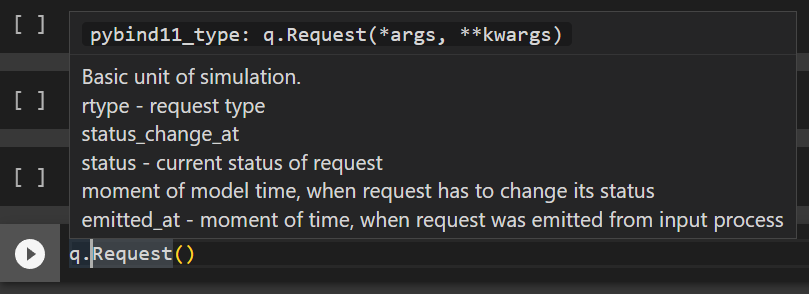
\includegraphics[scale=0.9, width=\textwidth]{doc_example.png}
	\caption{Пояснение к структуре Request}
	\label{doc_example}
\end{figure}


Помимо этого, важно отметить, что при привязке требуется указать, как именно будет происходить распоряжение памятью при создании и удалении объектов. В Python все переменные являются указателями, которые содержат в себе счетчик ссылок, означающий количество ссылающихся указателей на область в памяти. Как только счетчик становится равным нулю, объект уничтожается интерпретатором, что может повлечь за собой различного рода ошибки доступа к памяти и ее утечку. Во избежание перечисленных ошибок Pybind11 позволяет указать время жизни объекта, являющегося аргументом и возвращаемым значением по принципу Nurse--Patient:
 
 \lstset{language=C++,
 	basicstyle=\linespread{0.8}\ttfamily,
 	caption={Указание времени жизни объекта и тип возращаемого значения в Pybind11},
 	label={py_router_keep_alive_listing}
 }
 \begin{lstlisting}
 	py::class_<Router>(m, "Router", "Request queue")
 	.def("add_reader", &Router::AddReader, "reader"_a, "label"_a, py::keep_alive<1, 2>(), "Add request reader")
 	.def("reader_at", &Router::ReaderAt, py::keep_alive<1, 0>(), py::return_value_policy::reference, "get reader")
 \end{lstlisting}

В листинге \ref{py_router_keep_alive_listing} для метода add\_reader указано выражение py::keep\_alive<1, 2>(), что означает следующее: аргумент метода reader (индекс 2) не должен удалятся, пока не удален вызывающий метод объект (индекс 1). Данное выражение предотвратит ситуацию, когда аргумент reader может быть удален из памяти еще до того, как попадет в функцию add\_reader. Иными словами, выражение keep\_alive<$i,j$> указывает, что объект $j$ должен прожить хотя бы столько же, сколько проживет объект $i$. Индексом, равным единице, всегда является вызывающий объект; последующие индексы относятся к аргументам; индекс, равный нулю, означает возвращаемое значение функции. Пример использования указания времени жизни возвращаемого значения можно наблюдать в привязке метода reader\_at: поскольку данный метод является аналогом оператора индексации, крайне важно, чтобы ссылка на объект, возвращаемая методом не была удалена при обращении. Также для этого же метода указана политика возвращаемого значения --- reference. Это означает, что при возращении значения из функции управление данным объектом не переходит к Python, и ответственным за своевременное удаление объекта из памяти является код на стороне C++.

Для корректной строковой репрезентации объектов пакета используется атрибут Python--объектов под названием \_\_repr\_\_, так как по умолчанию объекты классов, принадлежащие стороне C++ будут отображаться в формате\\ <module.class\_name object at <адрес в памяти> >.

\subsection{Интеграция в процесс исследования}
После успешной компиляции проекта становится возможным использовать программу как нативный пакет Python, что и позволяет встроить ее непосредственно в среду, где проводятся исследования. Зачастую аналитические результаты, полученные при помощи математического аппарата, проверяются при помощи моделирования, однако производится оно на крайне малой выборке --- 2-3 запуска имитационной модели для получения совпадений в показателях. Причиной в том числе является подход к процессу запуска моделей. Как правило, их нужно сконфигурировать в специализированном ПО, провести моделирование, экспортировать результаты, импортировать их в среду для анализа и только далее приступить непосредственно к анализу. Также для него могут понадобится и сами конфигурации моделей. Подобный трудоемкий процесс является препятствием для получения достоверных результатов численными методами и отнимает большое количество времени на утилитарные действия. Наличие всех необходимых инструментов в одной среде значительно упрощает задачу проведения крупномасштабных экспериментов. Python используется \cite{mckinney2012python} во многих областях науки как инструмент исследования. В особенности это касается анализа данных, так как для него реализован ряд зарекомендовавших себя программных пакетов --- Pandas \cite{mckinney2011pandas}, позволяющий работать с данными в табличном виде и производить различные манипуляции и расчеты на их основе; NumPy \cite{numpy} --- пакет функций линейной алгебры и утилит для работы с многомерными данными; scikit-learn \cite{hackeling2017mastering} --- пакет для машинного обучения и статистического анализа; Scipy \cite{virtanen2020scipy} --- пакет, содержащий различные вычислительные алгоритмы и функции, и множество других. Таким образом, проведение моделирования на основе программного пакета Python предоставляет ряд преимуществ в удобстве, скорости и вычислительных возможностях.

С технической точки зрения данное решение также избавляет от необходимости реализации специальных классов для инстанциирования объектов с применением порождающих шаблонов проектирования (таких, как абстрактная фабрика \cite{fowler1997analysis}. В свою очередь процесс работы был вдохновлен известной библиотекой для машинного обучения PyTorch \cite{pytorch}, где модель, в данном случае нейронная сеть, предварительно составляется из набора слоев требуемой конфигурации и уже в последствии обучается. Попытка использовать подобный принцип была сделана и в случае имитационной модели, где аналогичным образом для начала создается пустая модель, не содержащая элементов, затем ими наполняется и конфигурируется: 
 \lstset{language=Python,
	basicstyle=\linespread{0.8}\ttfamily,
	caption={Указание времени жизни объекта и тип возращаемого значения в Pybind11},
	label={python_example}
}
\begin{pyin} [pyexampleinit]
from q_analysis import simulation as q
model = rq.Model()
model.set_time(0) 
model.set_end(1000000)
\end{pyin}
Добавление элементов:
\begin{pyin}[pyexampleaddproducers]
model.add_producer(rq.SimpleInput(rq.ExponentialDelay(1.1),0,0),"input")
model.add_producer(rq.SimpleInput(rq.ExponentialDelay(0.6),1,0),"call")
model.add_producer(rq.Orbit(rq.ExponentialDelay(0.81)),"orbit")
model.add_producer(
             rq.RqtNode(rq.ExponentialDelay(1.3),
             rq.ExponentialDelay(1)),"node")
\end{pyin}

\begin{pyin}[pyexampleaddconnections]
nodein = model.add_connection("input","out_slot","node","in_slot")
model.add_connection("call","out_slot","node","call_slot")
model.add_connection("orbit","out_slot","node","orbit_slot")
output = model.add_hanging_output_noqueue("node","out_slot")
model.add_connection("node","orbit_append_slot","orbit","in_slot")
\end{pyin}

\begin{pyin}[pyexampleaddreaders]
model.router_at(output).add_reader(rq.TimeCounter(),"count")
\end{pyin}

В ячейке \ref{pyexampleinit} производится создание модели и задание времени моделирования. Далее, в ячейке \ref{pyexampleaddproducers}, производится добавление элементов в модель:
\begin{itemize}
\item простейший поток с экспоненциально распределенными моментами порождения заявок, интенсивностью $1.1$ и меткой \textquote{input};
\item простейший поток с экспоненциально распределенными моментами порождения заявок, интенсивностью $0.6$ и меткой \textquote{call} в качестве источника вызываемых заявок;
\item орбита с интенсивностью повторного обращения заявок $0.81$ и меткой \textquote{orbit};
\item обслуживающий прибор с повторными обращениями и обратной связью, обрабатывающий входящие заявки в течение экспоненциально распределенной задержки с интенсивностью $1.3$ и вызываемые заявки в течение экспоненциально распределенной задержки с интенсивностью $1$. Имеет метку \textquote{node}.
\end{itemize}

Важно отметить, что для начала использования программного пакета достаточно установить его при помощи пакетного менеджера Python --- pip \cite{pip}. После этого он готов к работе, и его потребуется лишь импортировать, как это и проиллюстрировано в ячейке \ref{pyexampleinit}. Такая простота установки обеспечивается специальном форматом предварительно собранных пакетов Python --- wheel \cite{wheel}, экземпляр которого создается в результате компиляции и сборки программного пакета при помощи утилиты setuptools \cite{setuptools}. В последствии, для установки пакета из формата wheel не потребуется наличие исходного кода, компилятора или всей цепочки инструментов, использовавшихся при сборке, что позволяет легко распространять пакет и использовать его.

В ячейке \ref{pyexampleaddconnections} производится маршрутизация заявок между элементами модели:
\begin{itemize}
	\item заявки из входящего потока \textquote{input} попадают на прибор \textquote{node};
	\item заявки из источника вызываемых заявок \textquote{call} попадают на прибор \textquote{node};
	\item заявки, находящиеся на орбите \textquote{orbit} пытаются попасть обратно на прибор \textquote{node};
	\item заявки, не сумевшие захватить прибор \textquote{node} отправляются на орбиту \textquote{orbit};
	\item заявки, успешно обработанные прибором \textquote{node} отправляются в тупик.
\end{itemize}

В ячейке \ref{pyexampleaddreaders} к маршрутизатору, который представлен как тупик для обслуженных заявок, добавляется сборщик моментов прохождения заявок через маршрутизатор \textquote{count}. После этого модель готова к запуску и графически может быть представлена как изображено на рисунке \ref{py_example_model}.

\begin{figure}[H]
	\centering
	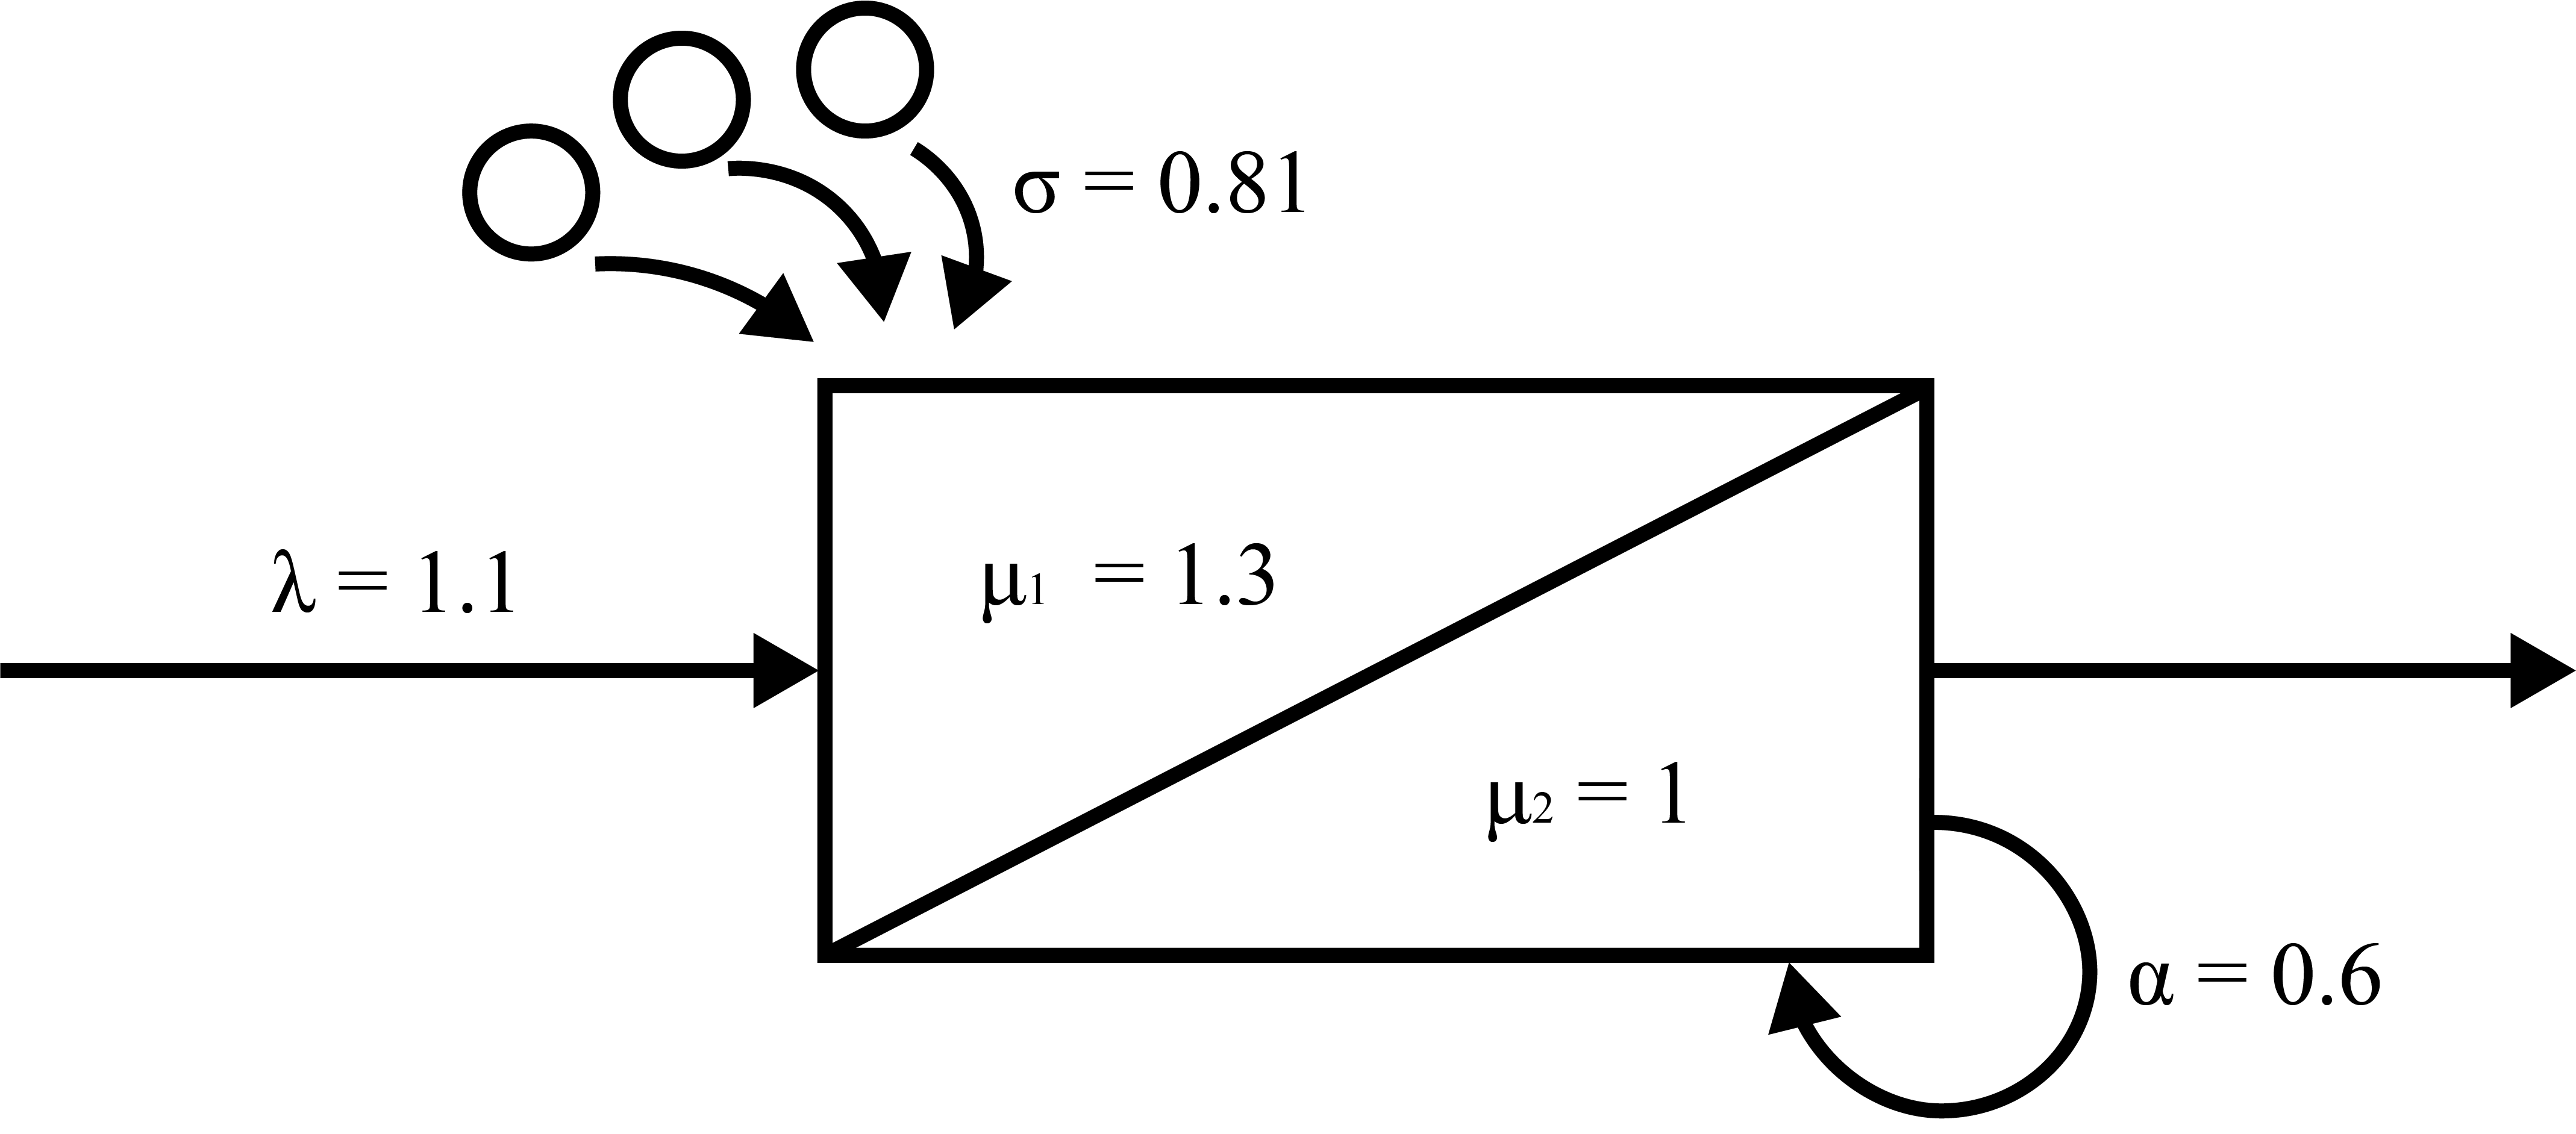
\includegraphics[scale=0.45]{2_sim_example.png}
	\caption{Пример составленной модели}
	\label{py_example_model}
\end{figure}
 
Таким образом, реализация программного пакета в качестве библиотеки для Python позволяет проводить численные эксперименты непосредственно в среде, где проводится статистический анализ, апробация результатов и остальные аспекты исследования.
\clearpage